\chapter{Introduction}
\label{sec:intro}

At the heart of programming languages
 lies the question of how to represent and manipulate programs.
Nearly all aspects of programming language work---including
 theorem proving, optimizing compilers, and program synthesis---%
 depend on these fundamental notions,
 since they dictate
 how (and how efficiently!) a tool
 stores and works with programs.
The choice of how to represent and manipulate programs
 largely determines the the efficacy of a tool or technique.

This thesis takes a fresh look at a data structure called the
 \textit{\egraph}~\cite{nelson}
 and a technique called \textit{\eqsat}~\cite{eqsat}
 for representing and manipulating programs, respectively.
Together,
 they offer great promise over the status quo of
 syntax trees and term rewriting,
Unfortunately,
 poor scalability and flexibility
 has limited the approach's reach.
% Unfortunately,
%  \egraphs (as described in 1980)
%  are not specifically tailored to the needs of
%  equality saturation (as described in 2009).
% This mismatch between data structure and algorithm
%  has led to poor scalability and flexibility,
%  limiting the approach's applicability.
 % have led \egraphs to
 % remain niche data structures (outside of theorem prover internals)
 % and limited \eqsat's applicability.

To bring \egraphs and \eqsat into
 the programming language practitioner's toolbox,
 % as a fast, flexible way to work with programs in
 % various domains,
 this thesis makes the following claim:
\begin{quote}
    \it\Thesisstmt
\end{quote}

The rest of this document
 supports that claim up in
 three ways:
\begin{enumerate}
\item
Our original research contributions presented in
 \autoref{sec:rebuild} and \autoref{sec:extensions}
 advance the state-of-the-art around
 \egraphs and \eqsat,
 enhancing both so that together they form a compelling
 alternative to conventional term rewriting.
\item
These theoretical advances
 are realized in \egg,
 a first-of-its-kind tool
 that has brought \egraphs and \eqsat
 to a wider range of users and domains than ever before.
\autoref{sec:egg} documents how \egg
 combines novel techniques with myriad practical niceties
 to make a generic, high-performance implementation of
 \egraphs and \eqsat.
\item
\autoref{sec:case-studies}
 makes an empirical case for the thesis statement
 in the form of published projects that rely on \egg.
These case studies demonstrate that \egraphs and \eqsat
 can now be used to
 achieve state-of-the-art results in various domains.
\end{enumerate}

\section{The World Before \egg}

Abstract syntax trees and
 directed term rewriting
 are (and will likely remain)
 the most popular approached
 for program representation and manipulation.
We defer discussion of issues with this approach to
 \autoref{sec:background}.
Here I would like to set the stage a little
 and describe the
 setting in which this
 thesis's contributions were made.

Equality graphs (\egraphs) were developed in late 1970s to
  efficiently represent congruence relations
  in automated theorem provers (ATPs).
At a high level, \egraphs~\cite{nelson, pp-congr}
  extend union-find~\cite{unionfind} to compactly represent
  equivalence classes of expressions while
  maintaining a key invariant:
  the equivalence relation is closed under congruence.\footnote{
    Intuitively, congruence simply means
    that $a \equiv b$ implies $f(a) \equiv f(b)$.}

\begin{figure}
  \centering
  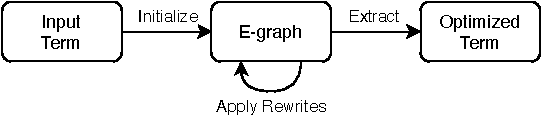
\includegraphics[width=0.6\linewidth]{eqsat}
  \caption{
    \Eqsat optimizes a program $p$ by storing it in an \egraph,
    growing the \egraph into a large set of equivalent terms
    by applying rewrites,
    and finally selecting the best program that is equivalent to $p$.
  }
  \label{fig:eqsat-flow}
\end{figure}

In the 2000s, work like Denali~\cite{denali} and
 the first equality saturation papers~\cite{eqsat, eqsat-llvm}
 began to repurpose \egraphs as the basis for program optimization.
% Over the past decade, several projects have repurposed \egraphs
%   to implement state-of-the-art, rewrite-driven
%   compiler optimizations and program synthesizers
%   using a technique known as \textit{equality saturation}~\cite{
%     denali, eqsat, eqsat-llvm, szalinski, yogo-pldi20, spores, herbie}.
Given an input program $p$,
  equality saturation constructs an \egraph $E$ that
  represents a large set of programs equivalent to $p$,
  and then extracts the ``best'' program from $E$.
The \egraph is grown by repeatedly applying
  pattern-based rewrites $\ell \to r$.
Each rewrite $\ell \to r$ includes
 a pattern $\ell$ to match and
 a pattern $r$ to instantiate and merge
 with the matched subterm.
Critically, these rewrites only add information\footnote{
  As opposed to traditional term rewriting which only considers a
    single term at a time.
  \autoref{sec:rewriting} covers this in detail.
}
  to the \egraph,
  eliminating the need for careful ordering.
Upon reaching a fixed point (\textit{saturation}),
  $E$ will represent \textit{all equivalent ways} to
  express $p$ with respect to the given rewrites.
After saturation (or timeout),
  a final extraction procedure
  analyzes $E$ and selects the
  optimal program according to
  a user-provided cost function.

Ideally, a user could simply provide
  a language grammar and rewrites,
  and equality saturation would produce a effective optimizer.
Three challenges blocked this ideal:
\begin{enumerate}
\item
Maintaining congruence can become expensive as $E$ grows.
In part, this is because \egraphs from the conventional ATP setting
  remained unspecialized to the distinct \textit{equality saturation workload}.
Early applications based on \eqsat had to limit
 their searches, which can impact the quality of results.
\item
Many applications critically depend on
  \textit{domain-specific analyses}, but
  integrating them required ad~hoc extensions to the \egraph.
The lack of a general extension mechanism
  forced researchers to re-implement
  equality saturation from scratch several times~\cite{herbie, eqsat, wu_siga19}.
\item
Even outside of the context of domain-specific analyses,
 the lack of a generic implementation of \egraphs and \eqsat
 made the ``just bring your grammar and rewrites'' vision impossible.
 Users had to start from scratch and reimplement state-of-the-art
  techniques for their own domain.
\end{enumerate}

\begin{wrapfigure}{r}{6cm}
  \centering
  \vspace{-22mm}
  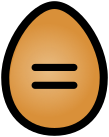
\includegraphics[width=3cm]{egg.png}
  \caption{The egg logo.}
  \label{fig:egg-logo}
  \vspace{-1em}
\end{wrapfigure}

\section{The \egg Era}

The work presented in this thesis
 addresses all of the concerns raised above.
Our theoretical contributions
 make \egraphs and \eqsat faster and more flexible,
 and \egg makes it all usable in real-world applications.

\paragraph{Equality Saturation Workload}

ATPs frequently query and modify \egraphs and
  additionally require the ability to
  undo modifications (e.g., in  DPLL(T)~\cite{dpll}).
This forces conventional \egraph designs
  to maintain the congruence invariant after every operation.
In contrast,
  the equality saturation workload
  can be factored into distinct phases of
  (1) querying the \egraph to simultaneously find all rewrite matches and
  (2) modifying the \egraph to merge in equivalences for all matched terms.

We present a new amortized algorithm
  called \textit{rebuilding} (\autoref{sec:rebuilding})
  that defers \egraph invariant maintenance
  to equality saturation phase boundaries without compromising soundness.
Empirically, rebuilding provides asymptotic speedups
  over conventional approaches.

\paragraph{Domain-specific Analyses}

Equality saturation is primarily driven by syntactic rewriting,
  but many applications require additional interpreted reasoning
  to bring domain knowledge into the \egraph.
Past implementations have resorted to
  ad~hoc \egraph manipulations
  to integrate what would otherwise be
  simple program analyses like constant folding.

To flexibly incorporate such reasoning,
  we introduce a new, general mechanism called \textit{\eclass analyses}
  (\autoref{sec:extensions}).
An \eclass analysis annotates each \eclass
  (an equivalence class of terms)
  with facts drawn from a semilattice domain.
%  resembling an abstract interpretation lifted to \egraphs.
As the \egraph grows,
  facts are introduced, propagated, and joined
  to satisfy the \textit{\eclass analysis invariant},
  which relates analysis facts to the terms represented in the \egraph.
Rewrites cooperate with \eclass analyses by
  depending on analysis facts and
  adding equivalences that in turn
  establish additional facts.
The examples and case studies
  demonstrate \eclass analyses like
  constant folding and free variable analysis
  which required bespoke customization in
  previous equality saturation implementations.

\paragraph{A generic, high-performance implementation}

We implement rebuilding and \eclass analyses in
  an open-source\footnote{
    \begin{tabular}[t]{ll}
      web: & \url{https://egraphs-good.github.io}\\
      source: & \url{https://github.com/egraphs-good/egg}\\
      documentation: & \url{https://docs.rs/egg}
    \end{tabular}
  }
  library called \egg (\textbf{e}-\textbf{g}raphs \textbf{g}ood).
\Egg specifically targets equality saturation,
  taking advantage of its workload characteristics and
  supporting easy extension mechanisms to
  provide \egraphs specialized for
  program synthesis and optimization.
\Egg also addresses more prosaic challenges,
  e.g., parameterizing over user-defined
  languages, rewrites, and cost functions
  while still providing an optimized implementation.
Our case studies in \autoref{sec:case-studies}
 demonstrate how \egg's features
 constitute a general, reusable \egraph library that can
 support equality saturation across diverse domains.

In summary,
 I believe that \eqsat has a big role in the future of programming
 languages.
When so many of the challenges to building programming tools
 revolve around \textit{choice},
 \eqsat's ability to operate over many terms \textit{simultaneously}
 is hard to ignore.
% offers an alternative to heuristics or backtracking
Even in situations where equality saturation is not the best approach,
 it may be the easiest,
 since it offloads work from the developer
 to the computer.
More complex applications may require
 making a particular choice at some points and
 taking all possible paths in others;
 \egg's practical, generic implementation is a compatible
 with this approach as well.

Fast and flexible \eqsat
 provides the power to \textit{not} choose how to manipulate
 programs,
 which can be a boon to both power users and
 domain experts who may not have expertise in building programming
 language tools.
I hope this thesis and \egg are steps toward
 having \egraphs and \eqsat in the toolbox
 of anyone working with programs,
 regardless of their expertise,
 the size and scale of the problem,
 or the application domain.


% In summary, the contributions of this paper include:
% \begin{itemize}
% \item Rebuilding (\autoref{sec:rebuilding}),
%   a technique that restores key correctness and performance invariants
%   only at select points in the equality saturation algorithm.
%   Our evaluation demonstrates that rebuilding is faster than
%   existing techniques in practice.

% \item \Eclass analysis (\autoref{sec:extensions}),
%   a technique for integrating domain-specific analyses
%   that cannot be expressed as purely syntactic rewrites.
%   The \eclass analysis invariant provides the guarantees
%   that enable cooperation between rewrites and analyses.

% \item A fast, extensible implementation of
%   \egraphs in a library dubbed \egg (\autoref{sec:impl}).

% \item Case studies of real-world, published tools that use \egg
%     for deductive synthesis and program optimization across domains such as
%     floating point accuracy,
%     linear algebra optimization,
%     and CAD program synthesis
%     (\autoref{sec:case-studies}).
%     Where previous implementations existed,
%       \egg is orders of magnitude faster and offers more features.
% \end{itemize}



%%% Local Variables:
%%% TeX-master: "../thesis"
%%% End:
